\documentclass{beamer}
%\usetheme{Madrid}
%\usetheme{Boadilla}
%\usetheme{default}
%\usetheme{Warsaw}
%\usetheme{Frankfurt}
\usetheme{Cesena}
%\usetheme{Bergen}
%\usetheme{Hannover}
%\usecolortheme{dolphin}
%\usetheme{Darmstadt}
%\setbeamertemplate{footline}[page number]
%\setbeamercovered{transparent}
%\setbeamercovered{invisible}
% To remove the navigation symbols from
% the bottom of slides

\usepackage{graphicx}
\usepackage[english]{babel}
\usepackage[utf8]{inputenc}
\usepackage{listings}
\usepackage{xcolor}

%\usepackage{url}

%\usepackage[pdftex,bookmarks,colorlinks,%
%pdfauthor={Daniele Bellavista},%
%pdftitle={Shellcoding, and introduction},%
%pdftex]{hyperref}
%\usepackage{bm}  % For typesetting bold math (not \mathbold)

\title[]{Hovering Information System using MAS}

\author[]{Daniele Bellavista}

\institute[University of Bologna]
{
\emph{University of Bologna, Scuola di Ingegneria ed Architettura}\\
\emph{Sistemi MultiAgente LM 2012/2013}
}

\begin{document}

{
	\setbeamertemplate{footline}{}
	\setbeamertemplate{navigation symbols}{}
	\begin{frame}
	  \titlepage
	\end{frame}
}

\begin{frame}{Outline}
\tableofcontents
\end{frame}

\begin{frame}{Hovering Information System}
	\section{HIS}
	\begin{block}{Introduction}
		\begin{itemize}
			\item Bla bla bla
		\end{itemize}
	\end{block}
\end{frame}

\begin{frame}
	\begin{figure}
		\centering
		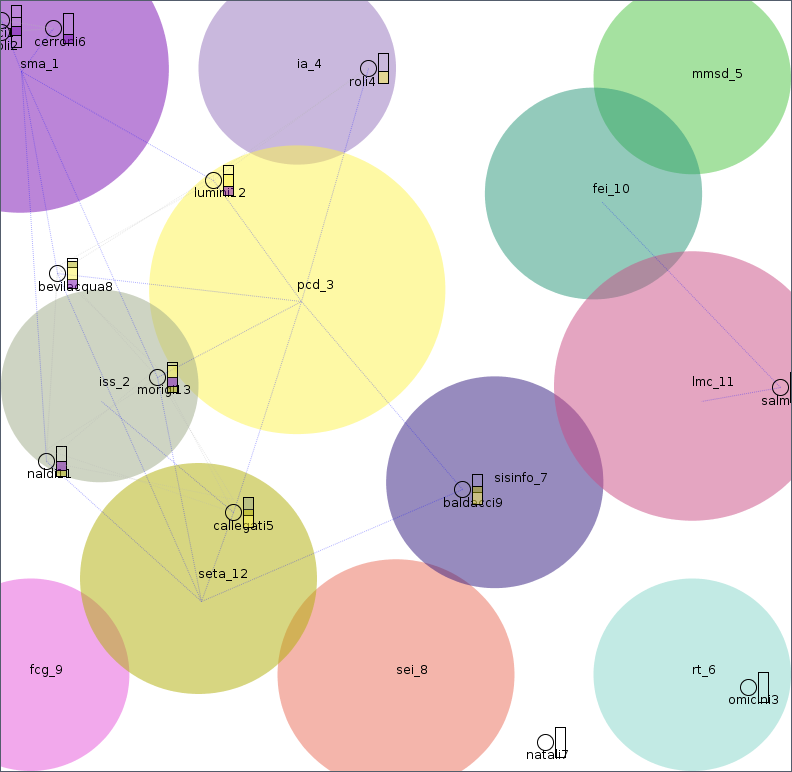
\includegraphics[height=\textheight]{../imgs/screen1.png}
		\caption{Screenshot 1}
		\label{fig:screens1}
	\end{figure}
\end{frame}


\end{document}
